\documentclass[french,a4paper,addpoints,11pt]{exam}
\usepackage{hexercises}
\usepackage{amsmath}
\usepackage[french]{babel}
\usepackage{siunitx}
\usepackage{multicol}

\DeclareSIUnit{\perthousand}{\text{\textperthousand}}

\makeatletter
\renewcommand{\maketitle}{\@maketitle}
\makeatother

\title{Freinage d'une voiture avec traînée aérodynamique}
\seriesno{\texttt{0xe1}}
\department{TIN}
\classroom{INFO1-TIN}

\setlength\answerlinelength{10 cm}
\setlength\answerskip{3ex}
\setlength\answerclearance{1.1ex}
\CorrectChoiceEmphasis{}
\renewcommand{\thepartno}{\alph{partno}}%
\renewcommand{\partlabel}{\thepartno.}%
\renewcommand{\arraystretch}{1.75}

\author{Yves Chevallier}

\begin{document}
\maketitle
\thispagestyle{headandfoot}

\begin{multicols}{2}
    \begin{questions}
        \question

        \section*{Modèle physique}

        \vskip 1em
        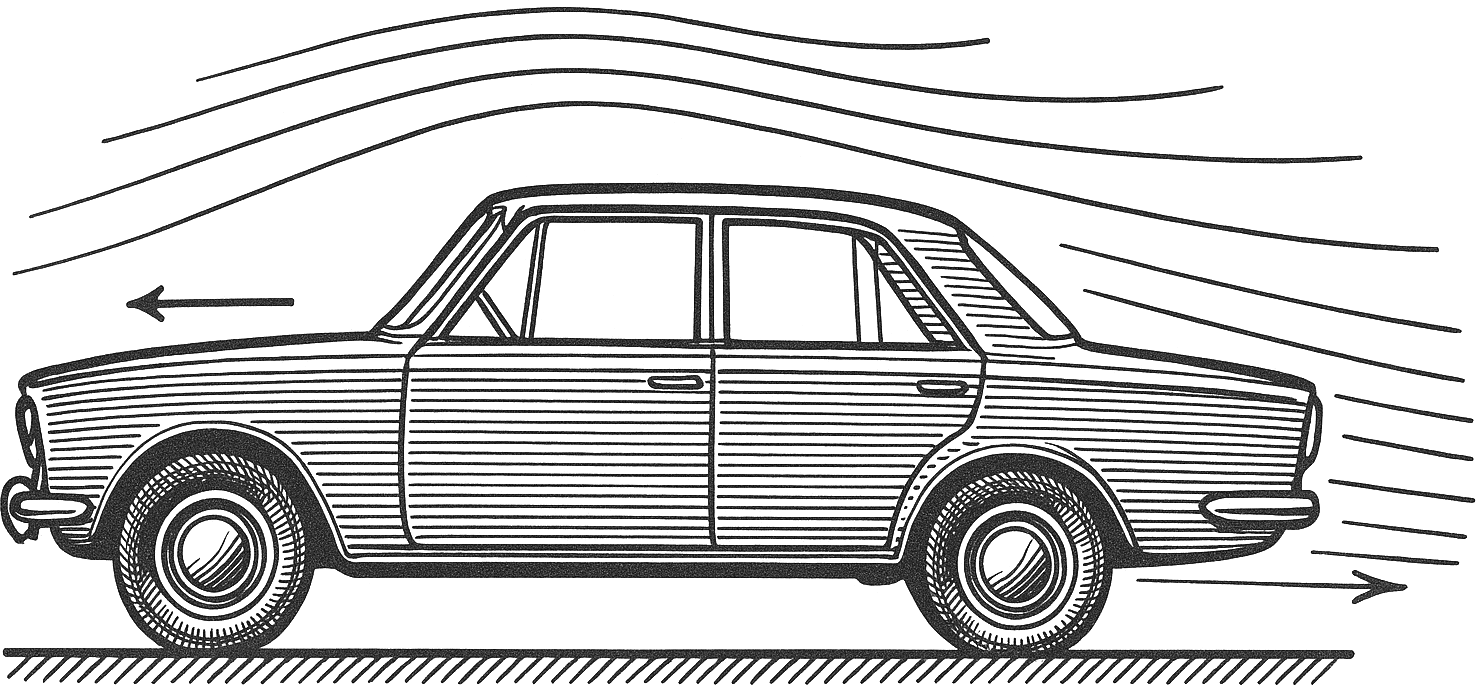
\includegraphics[width=\columnwidth]{car.png}
        On modélise le freinage d'une voiture par une décélération constante $a_0 = \mu g$ et une force de traînée aérodynamique quadratique
        $F_D = \tfrac{1}{2}\rho C_d A v^2$. On montre que la vitesse initiale $v_0$ mène aux formes fermées suivantes, avec
        \[ k = \frac{\rho C_d A}{2m}. \]

        Le temps d'arrêt vaut :
        \[
            t_{\text{stop}} = \frac{1}{\sqrt{a_0 k}}\,\arctan\!\left(v_0\sqrt{\tfrac{k}{a_0}}\right)
        \]
        et la distance d'arrêt vaut :
        \[
            x_{\text{stop}} = \frac{1}{2k}\,\ln\!\left(1 + \tfrac{k}{a_0}v_0^2\right).
        \]

        Toutes les grandeurs doivent être exprimées en unités SI cohérentes, soit :
        \begin{itemize}
            \item $m$ en kilogrammes (kg),
            \item $A$ en mètres carrés (m\textsuperscript{2}),
            \item $\rho$ en kilogrammes par mètre cube (kg·m\textsuperscript{$-3$}),
            \item $g$ en mètres par seconde carrée (m·s\textsuperscript{$-2$}),
            \item $v_0$ en mètres par seconde (m·s\textsuperscript{$-1$}).
        \end{itemize}



        \section*{Cahier des charges}

        Écrire un programme \texttt{brake.c} qui lit \textbf{sept arguments} en \texttt{int} ou \texttt{double} depuis la ligne de commande, donnés dans des unités volontairement peu pratiques. On suggère d'utiliser un suffixe dans le nom des variables pour rappeler l'unité, par exemple \texttt{v0\_kmh} pour la vitesse initiale en km/h. Les arguments sont :

        \begin{enumerate}
            \item \texttt{v0\_kmh} : vitesse initiale en \si{\kilo\metre\per\hour};
            \item \texttt{m\_t} : masse du véhicule en tonnes;
            \item \texttt{mu\_permille} : coefficient de frottement en \si{\perthousand};
            \item \texttt{A\_dm2} : surface frontale en \si{\deci\metre\squared};
            \item \texttt{Cd} : coefficient de traînée (sans dimension);
            \item \texttt{rho\_gL} : densité de l'air en g/L (indice : \SI{1}{\gram\per\litre} = \SI{1}{\kilogram\per\metre\cubed});
            \item \texttt{g\_Gal} : accélération gravitationnelle en Gal (\SI{1}{Gal} = \SI{0.01}{\metre\per\second\squared}).
        \end{enumerate}

        Le programme doit :
        \begin{enumerate}
            \item convertir \textbf{toutes} les grandeurs en unités SI ;
            \item calculer successivement $a_0$, $k$, $t_{\text{stop}}$ et $x_{\text{stop}}$ ;
            \item afficher les résultats avec trois décimales, en secondes pour le temps et en mètres pour la distance.
        \end{enumerate}

        \section*{Exemple d'exécution}

        \begin{lstlisting}
$ ./freinage 130 1.4 800 22 0.30 1.225 981
Temps d'arrêt : 4.594 s
Distance d'arrêt : 82.881 m
        \end{lstlisting}

        \section*{Déroulement conseillé}
        \begin{enumerate}
            \item Réfléchir au problème, aux conversions et aux formules.
            \item Écrire un squelette de programme avec les inclusions nécessaires et la fonction \texttt{main}.
            \item Lire les arguments et vérifier le nombre attendu ; quitter proprement sinon.
            \item Implémenter les conversions et vérifier les valeurs intermédiaires au besoin.
            \item Calculer les grandeurs physiques et valider avec l'exemple fourni.
            \item Formater l'affichage des résultats avec trois décimales.
        \end{enumerate}

        \begin{solution}
\begin{lstlisting}[language=C]
#include <math.h>
#include <stdbool.h>
#include <stdio.h>
#include <stdlib.h>

static bool is_valid(double v0, double m, double mu,
                     double A, double Cd, double rho, double g) {
    return v0 >= 0 && m > 0 && mu >= 0 && A > 0 && Cd >= 0 && rho > 0 && g > 0;
}

int main(int argc, char *argv[]) {
    if (argc != 8) {
        fprintf(stderr,
                "Usage: %s v0_kmh m_t mu_permille A_dm2 Cd rho_gL g_Gal\n",
                argv[0]);
        return EXIT_FAILURE;
    }

    const double v0_kmh = atof(argv[1]);
    const double m_t = atof(argv[2]);
    const double mu_permille = atof(argv[3]);
    const double A_dm2 = atof(argv[4]);
    const double Cd = atof(argv[5]);
    const double rho_gL = atof(argv[6]);
    const double g_Gal = atof(argv[7]);

    const double v0 = v0_kmh * (1000.0 / 3600.0);
    const double m = m_t * 1000.0;
    const double mu = mu_permille / 1000.0;
    const double A = A_dm2 * 0.01;
    const double rho = rho_gL;
    const double g = g_Gal * 0.01;

    if (!is_valid(v0, m, mu, A, Cd, rho, g)) {
        fputs("Arguments physiques invalides.\n", stderr);
        return EXIT_FAILURE;
    }

    const double a0 = mu * g;
    const double k = (rho * Cd * A) / (2.0 * m);
    const double t_stop = (1.0 / sqrt(a0 * k)) * atan(v0 * sqrt(k / a0));
    const double x_stop = (1.0 / (2.0 * k)) * log(1.0 + (k / a0) * v0 * v0);

    printf("Temps d'arrêt : %.3f s\n", t_stop);
    printf("Distance d'arrêt : %.3f m\n", x_stop);
    return EXIT_SUCCESS;
}
\end{lstlisting}
        \end{solution}
    \end{questions}
        \end{multicols}
\end{document}
